\subsection{Segment Identification Using $\theta_{\sat}$ \label{sec::segment_id}}

With $\hat\theta_{\sat}$ estimated, the saturated model response
$\hat\eta_{\sat}(k) = \phi_{\sat}^T(k)\,\hat\theta_{\sat}$ is computed for each time step. A data point is classified
as near-saturated if the prediction error is small:
\begin{align}
    \abs{\hat\eta_{\sat}(k) - \eta(k)} \leq \varepsilon_{\sat} \implies \text{saturated operation}
    \label{eqn::sat_detect}
\end{align}
The threshold $\varepsilon_{\sat}$ is chosen from the variance of the prediction error distribution
($\varepsilon_{\sat} = 2.5\times 10^{-3}\, mol/m^{3}$ for the test-cell dataset). The saturated model response depends
only on $u_1$, $F$, and $T$ (not on the previous state or urea dosing), so it can be evaluated without simulation.

\begin{figure}[!ht]
    \centering
    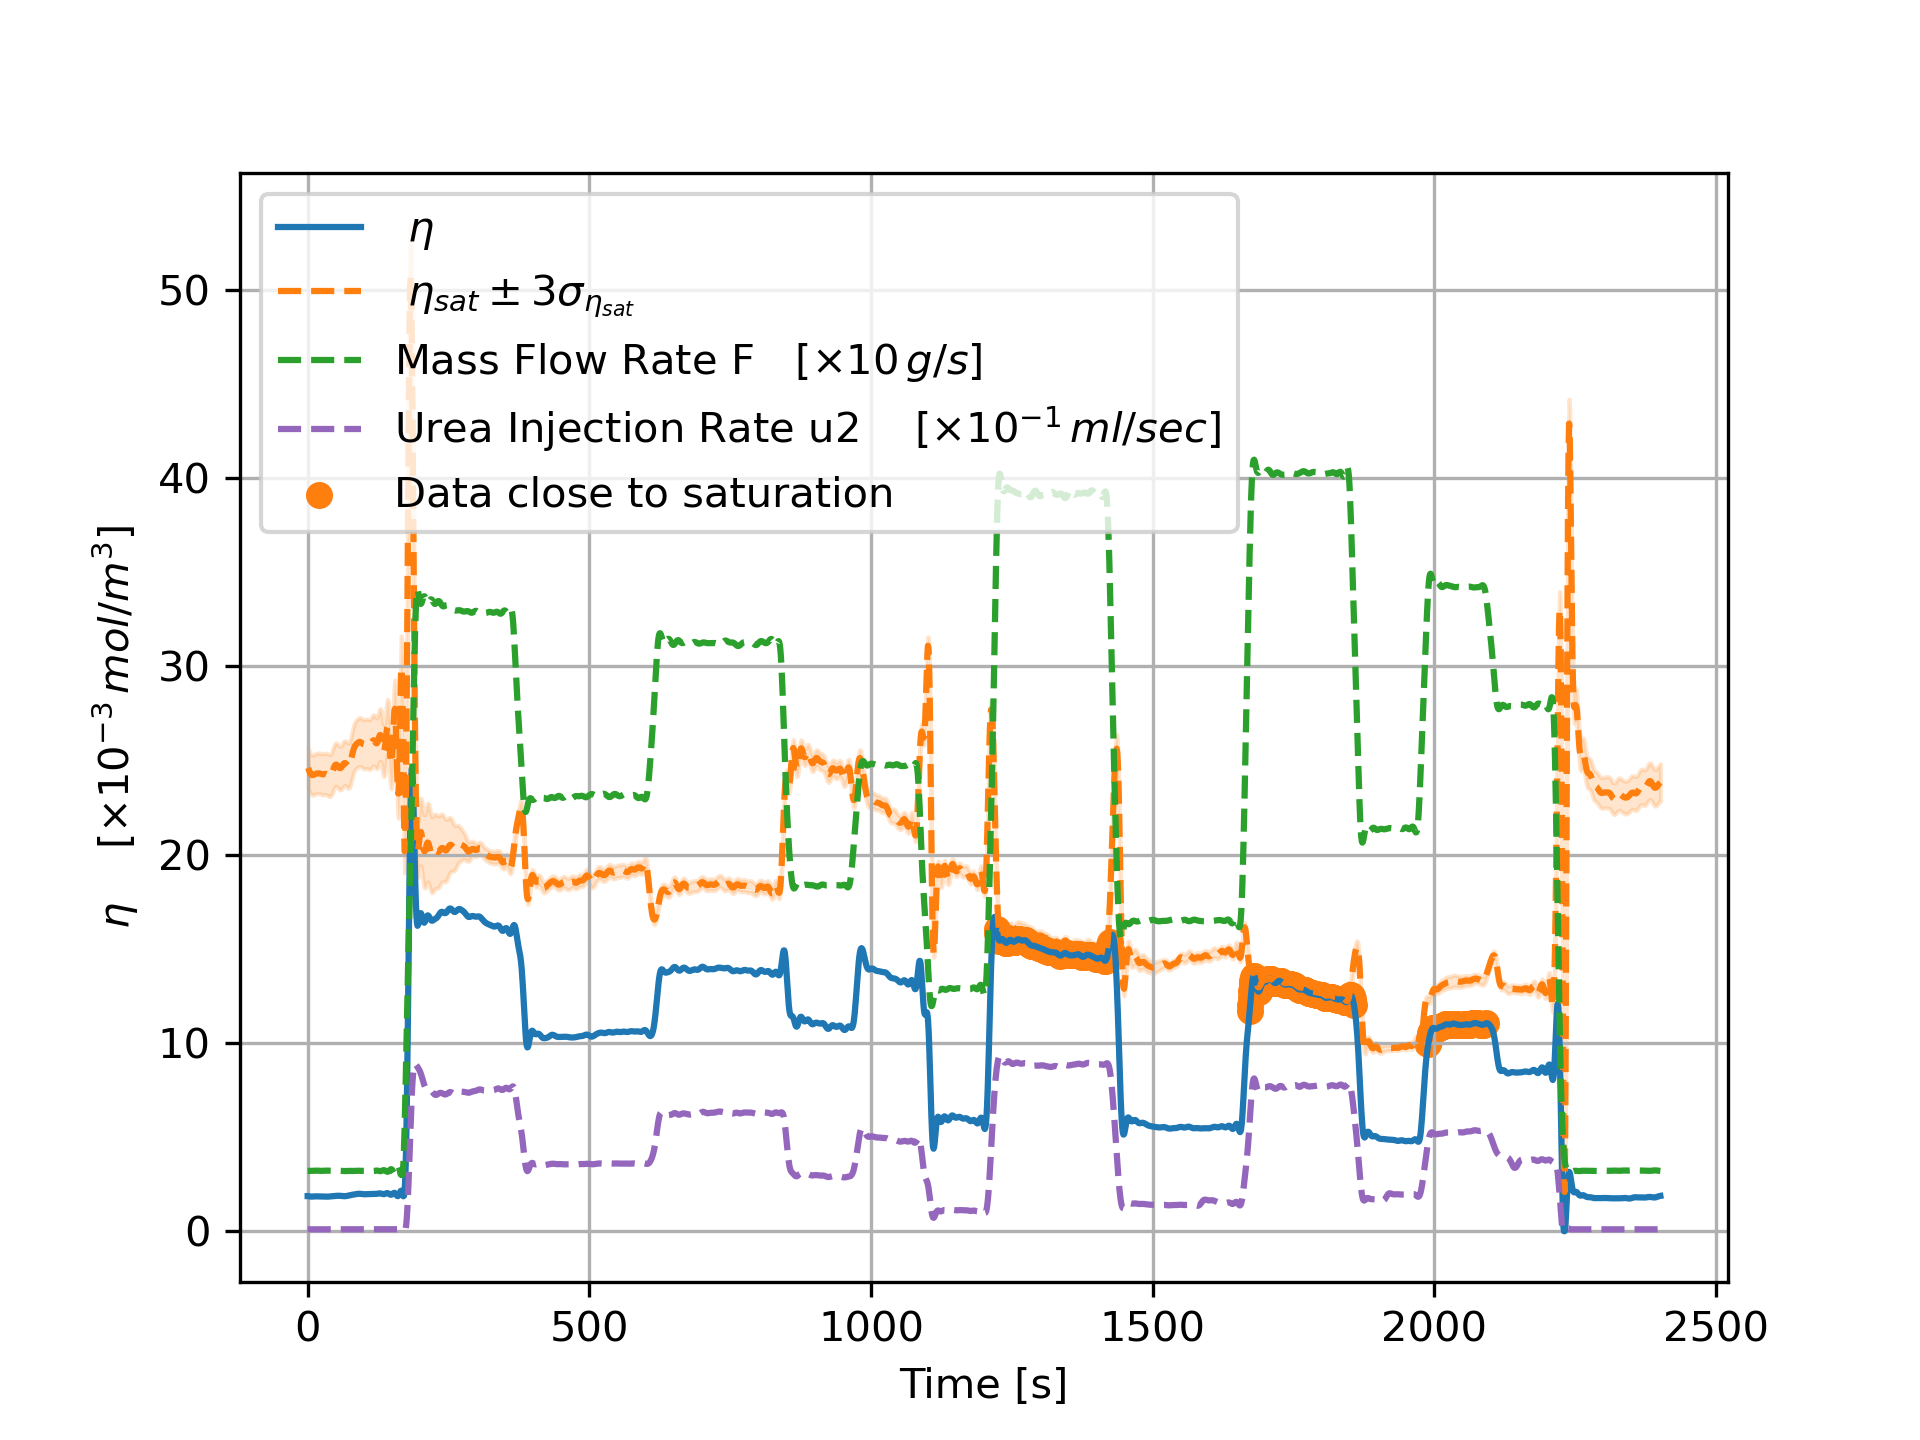
\includegraphics[width=\figWidth]{./figs/3-sysID/SatDetect_dg_rmc_1_FTIR.png}
    \caption{Catalyst mode detection for degreened RMC test-cell data}
    \label{fig::cat_mode_det}
\end{figure}

\begin{table}[!ht]
    \centering
    \caption{Data points close to catalyst saturation}
    \label{tab::sat_data_perc}
    \begin{tabular}{l r r r}
        \hline \hline
        Test & $N$ & $N_{\sat}$ (FTIR) & $N_{\sat}$ ($\nox$ sensor) \\
        \hline \hline
        DG RMC 1     & 2402 & 490 & 492 \\
        DG RMC 2     & 2402 & 493 & 494 \\
        DG RMC 3     & 2402 & 491 & 493 \\
        Aged RMC     & 2402 & 515 & 515 \\ \hline
        DG Hot FTP 1 & 634  & 186 & 194 \\
        DG Hot FTP 2 & 634  & 181 & 191 \\
        DG Hot FTP 3 & 638  & 180 & 198 \\
        Aged Hot FTP & 636  & 198 & 220 \\
        \hline \hline
    \end{tabular}
\end{table}

The unsaturated segments (the complement) are used for $\theta_{\nox}$ estimation in the next subsection.
